\documentclass[]{article}
% used packages
\usepackage[german]{babel}   % enables umlaute
\usepackage[utf8]{inputenc}  % set encoding to utf8 otherwise no umlaute
\usepackage{graphicx}        % for including graphics
\usepackage[hidelinks]{hyperref}        % for using hyperlinks in the document
\usepackage{tabularx}        % for extending tabluar
\usepackage{multirow}        % for rowspan in tabularx
\usepackage{ltablex}         % tables over multiple pages
\usepackage{textcmds}        % for quote support
\usepackage{pdfpages}        % for pdf include
\usepackage{caption}
\usepackage{minted}
\usepackage{listings}
\usepackage[left=1.0in, right=1.0in, top=1.0in, bottom=1.0in]{geometry} % for custom page layout

% Title Page
\title{Raspberry PI Security Application}
\author{Thonas Herzog, Philipp Wurm}


\newcommand{\imageDir}{../images}
\newcommand{\srcDir}{../example-src}
\newcommand{\dockerTestDir}{../../java/testsuite/client/src/main/resources/docker}
\newcommand{\dockerRPIDir}{../../host/docker}
\renewcommand\listingscaption{Quelltext}

\newenvironment{code}{\captionsetup{type=listing}}{}

\newmintedfile[yamlFile]{yaml}{
	linenos=true, 
	frame=single, 
	breaklines=true, 
	tabsize=2,
	numbersep=5pt,
	xleftmargin=10pt,
	baselinestretch=1,
	fontsize=\footnotesize
}

\newmintedfile[javaFile]{java}{
	linenos=true, 
	frame=single, 
	breaklines=true, 
	tabsize=2,
	numbersep=5pt,
	xleftmargin=10pt,
	baselinestretch=1,
	fontsize=\footnotesize
}

\begin{document}
\maketitle

\section{Einleitung}
Diese Dokument stellt die Dokumentation des Projekts \emph{Raspberry PI Security}, in weiterer Folge \emph{RPISec} genannt, dar, welches für die Lehrveranstaltung \emph{Mobile und ubiquitäre Systeme} realisiert wurde. In diesem Projekt wird eine Heimsicherheitsanwendung mit einem \emph{Raspberry PI 3 Model B}, \emph{Docker} und \emph{Spring Boot Microservices} umgesetzt, das bei einem Sicherheitsverstoß in der Lage sein soll, bekannte mobile Endgeräte von registrierten Benutzern über diesen Sicherheitsverstoß zu informieren. 

\subsection{Problemdarstellung}
Dieser Abschnitt behandelt die Problemdarstellung, welche die Grundlage für das umzusetzende Projekt \emph{RPISec} ist. Bei einem Auslösen eines an dem \emph{Raspberry PI} angeschlossenen Bewegungssensors,  sollen alle am System registrierten Benutzer über ihre mobilen Endgeräte wie Handy oder Tablet über den Vorfall informiert werden, sowie die Möglichkeit haben ein Bild zu erhalten, welches den Sicherheitsbereich zum Zeitpunkt des Sicherheitsverstoßes zeigt. 
\newline
\newline
Da es sich um eine Sicherheitsanwendung handelt, soll die Benutzerverwaltung sowie die Authentifizierung \emph{In-House} gehalten werden, also die Sicherheitsanwendung selbst soll in der Lage sein die Benutzer zu verwalten und die Authentifizierung der Benutzer durchzuführen. Da sich die mobilen Endgeräte in irgendwelchen Netzen an das Internet anbinden können, wie zum Beispiel über einen Mobilfunkanbieter, Internetanbieter oder öffentlichen \emph{Hot-Spot}, wird ein \emph{Messaging} Dienst benötigt, über den die mobilen Endgeräte erreicht werden können. Dieser \emph{Messaging} Dienst muss es erlauben, dass die Benutzerverwaltung extern erfolgen kann, da wir diesen \emph{Messaging} Dienst nicht vertrauen wollen und daher den \emph{Messaging} Dienst auch nicht die Benutzerverwaltung überlassen wollen. Ebenso wird ein online Speichermedium benötigt, dass alle gemachten Bilder speichert, damit die registrierten Benutzer jederzeit darauf zugreifen können.


\subsection{Funktionsweise}
Dieser Abschnitt behandelt die Funktionsweise von \emph{RPISec}. Die Abbildung \ref{fig:image-system-structure} zeigt den Systemaufbau von \emph{RPISec} mit der involvierten Hardware und \emph{Cloud} Diensten. 
\begin{figure}[h]
	\centering
	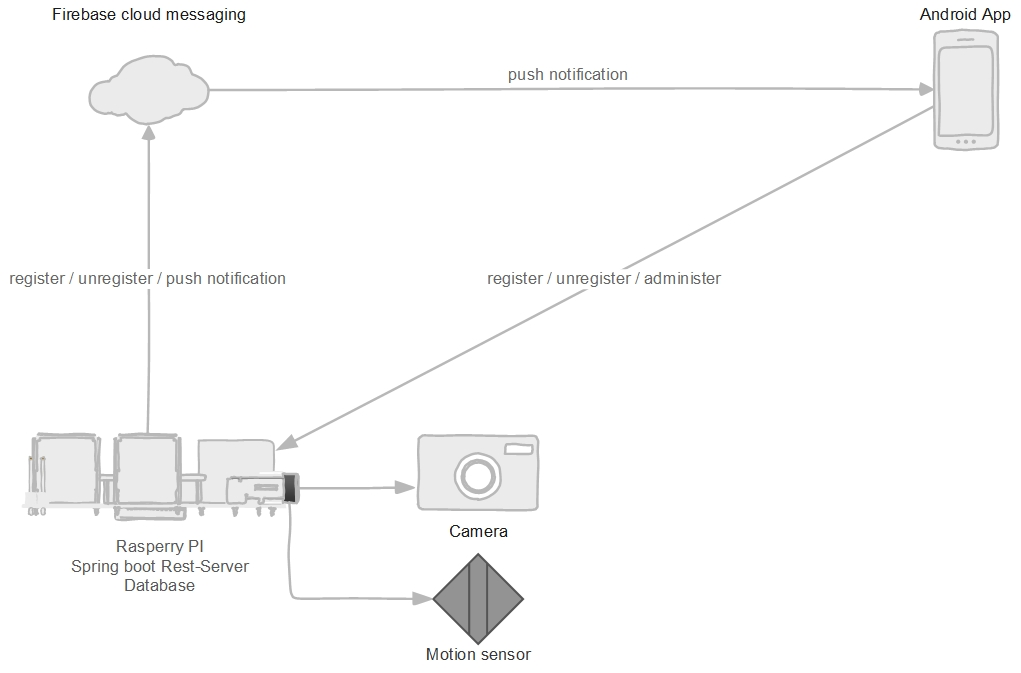
\includegraphics[scale=0.7]{\imageDir/Infrastructure.jpg}
	\caption{Systemaufbau der \emph{RPISec} Applikation}
	\label{fig:image-system-structure}
\end{figure}
\ \newpage

\subsubsection{Zugangsverifikation}
Beim Start des Systems wird vom Authentifizierungsservice \emph{(Auth-Service)} ein Administrator Benutzer erstellt, wenn dieser nicht bereits existiert. Ein neu angelegter Benutzer wird über eine E-Mail dazu aufgefordert, seinen Zugang zu aktivieren, in dem er ein Password vergibt. Im Idealfall würde die Zugangsverifikation nur im Heimnetz möglich sein.
\begin{figure}[h]
	\centering
	
\includegraphics[scale=0.5]{\imageDir/view-verify-account.JPG}
	\caption{Zugangsaktivierung}
	\label{fig:image-veriy-account}
\end{figure}
\begin{figure}[h]
	\centering
	
\includegraphics[scale=0.5]{\imageDir/view-verified-account.JPG}
	\caption{Bestätigung der Aktivierung}
	\label{fig:image-veriied-account}
\end{figure}

\subsubsection{\emph{Client Login}}
Die Abbildung \ref{fig:image-sequence-client-login} zeigt das Sequenzdiagramm, welches den Ablauf des Logins eines registrierten Benutzers über einen mobilen \emph{Client} beschreibt.
\begin{figure}[h]
	\centering
	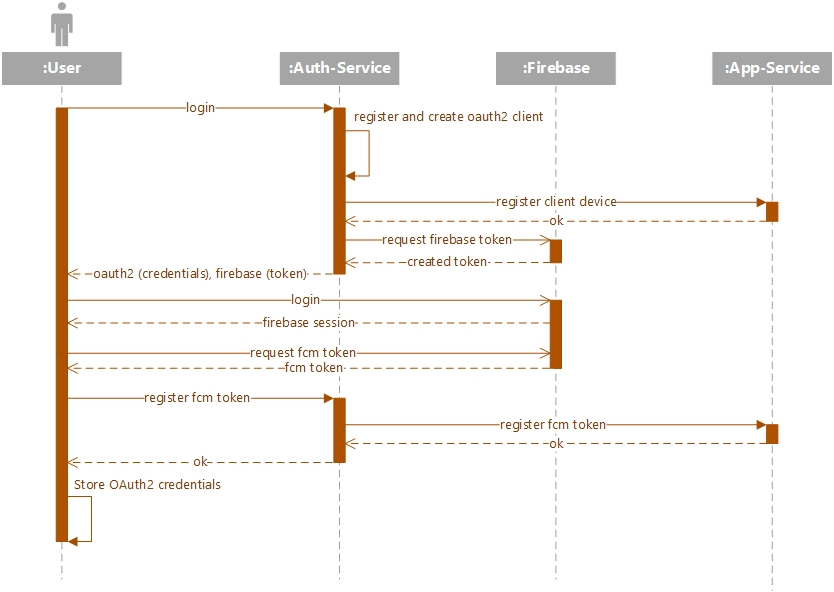
\includegraphics[scale=0.55]{\imageDir/sequence-client-login.jpg}
	\caption{Sequenzdiagramm des Benutzerlogins}
	\label{fig:image-sequence-client-login}
\end{figure}
\ \newpage
Im Zuge des Benutzerlogins wird der mobile \emph{Client} am \emph{(Auth-Service)}, der die Authentifizierung und Benutzerverwaltung verantwortlich ist und am Applikationsservice \emph{(App-Service)}, der mit der Hardware und dem \emph{Messaging} Dienst interagiert, registriert. Der \emph{Auth-Service} erstellt bei jedem Login einen neuen \emph{OAuth2-Client} und löscht gegebenenfalls einen bereits bestehenden  \emph{OAuth2-Client} für den aktuellen mobilen \emph{Client}. Das Erstellen eines \emph{OAuth2-Clients} für jeden mobilen \emph{Client} wird durchgeführt, da mit der \emph{Client}-Applikation keine \emph{Oauth2-Client} Zugangsdaten an die mobilen \emph{Clients} mit ausgeliefert werden sollen.
\newline
\newline
Dem mobilen \emph{Client} wird bei einem Login ein Authentifizierungstoken für den \emph{Cloud} Dienst übermittelt, mit dem sich der mobile \emph{Client} am \emph{Cloud} Dienst anmelden kann. Nachdem Login eines mobilen \emph{Clients} am \emph{Cloud} Dienst holt sich der mobile \emph{Client} seine eindeutige Id vom \emph{Cloud} Dienst in Form eines Tokens, der am \emph{Auth-Service} registriert wird, der wiederum den Token am \emph{App-Service} registriert, damit dieser in der Lage ist, Nachrichten an die registrierten mobilen \emph{Clients} zu versenden.  

\subsubsection{Sicherheitsverstoß melden}
\begin{figure}[h]
	\centering
	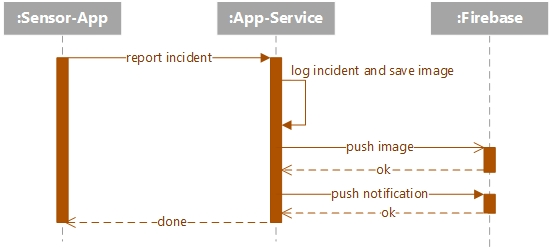
\includegraphics[scale=0.7]{\imageDir/sequence-incident.jpg}
	\caption{Sequenzdiagramm für das Behandelns eines Sicherheitsverstoßes}
	\label{fig:image-sequence-incident}
\end{figure}
\ \newline
Die Abbildung \ref{fig:image-sequence-incident} zeigt das Sequenzdiagramm für das Behandeln eines Sicherheitsverstoßes, der von der Sensorapplikation erkannt und dem Applikationsservice mitgeteilt wird. Der Sicherheitsverstoß wird über den \emph{Cloud} Dienst an die mobilen \emph{Clients} gemeldet, wobei einerseits eine Nachricht an die mobilen \emph{Clients} versendet wird, sowie das gemachte Bild in einer Onlinedatenbank den mobilen \emph{Clients} zum Download zur Verfügung gestellt wird. Die Benutzer können jederzeit auf die Onlinedatenbank zugreifen und sich die Bilder auf ihren jeweiligen mobilen \emph{Clients} herunterladen. 
\newline
\newline
Der Ansatz einen \emph{Cloud} Dienst zu verwenden sorgt dafür, dass das \emph{RPISec} System entlastet wird, da der Datenfluss und die Netzwerkzugriffe vom System ins Internet sowie umgekehrt minimiert werden. Die Daten müssen nur einmalig in die \emph{Cloud} hochgeladen werden und die Benutzer können jederzeit, beliebig oft und von jedem beliebigen mobilen \emph{Client} darauf zugreifen.
\newpage
 
\subsubsection{Nachrichtenempfang am mobilen \emph{Client}}
Die Abbildung \ref{fig:image-sequence-client-notification} zeigt den Ablauf einer Benachrichtigung eines mobilen \emph{Clients} über den \emph{Messaging} Dienst.
\begin{figure}[h]
	\centering
	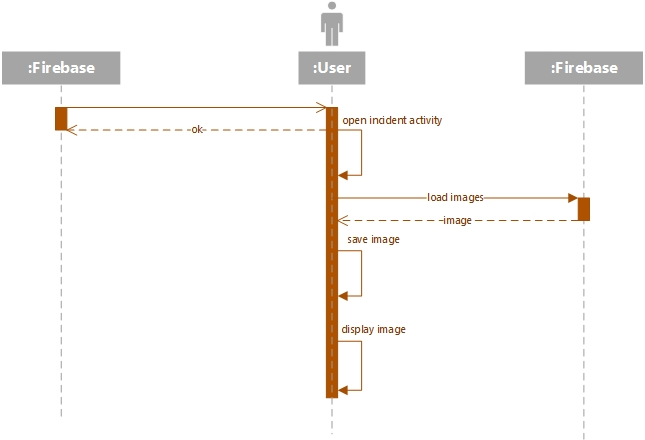
\includegraphics[scale=0.7]{\imageDir/sequence-client-notification.jpg}
	\caption{Sequenzdiagramm der Benachrichtigung eines mobilen \emph{Clients}}
	\label{fig:image-sequence-client-notification}
\end{figure}
\ \newline
Nachdem das System die mobilen \emph{Clients} via dem \emph{Messaging} Dienst über einen Sicherheitsverstoß benachrichtigt hat, erhalten die mobilen \emph{Client}-Anwendungen die Nachricht von dem \emph{Messaging} Dienst und zeigen diese an. Nachdem die Benutzer auf die Nachricht geklickt haben, wird eine \emph{Activity} für das Anzeigen der Bilder geöffnet, die alle bereits gespeicherten Bilder und das neu geladene Bild anzeigt. Diese Daten werden von der Onlinedatenbank bereitgestellt. 
\section{\emph{Raspberry PI}}
Dieser Abschnitt behandelt die verwendete Hardware für \emph{RPISec}. Für den Testaufbau wurden folgende Hardwarekomponenten verwendet.
\begin{itemize}
	\item Ein \emph{Raspberry PI 3 Model B}\footnote{\url{https://www.raspberrypi.org/products/raspberry-pi-3-model-b/}},
	\item \emph{AZDeliveryCamRasp}\footnote{\url{https://az-delivery.de/products/raspberrykamerav1-3}} und ein
	\item \emph{HC-SR501\footnote{\url{https://www.mpja.com/download/31227sc.pdf}} Bewegungssensor}.
\end{itemize}
\begin{figure}[h]
	\centering
	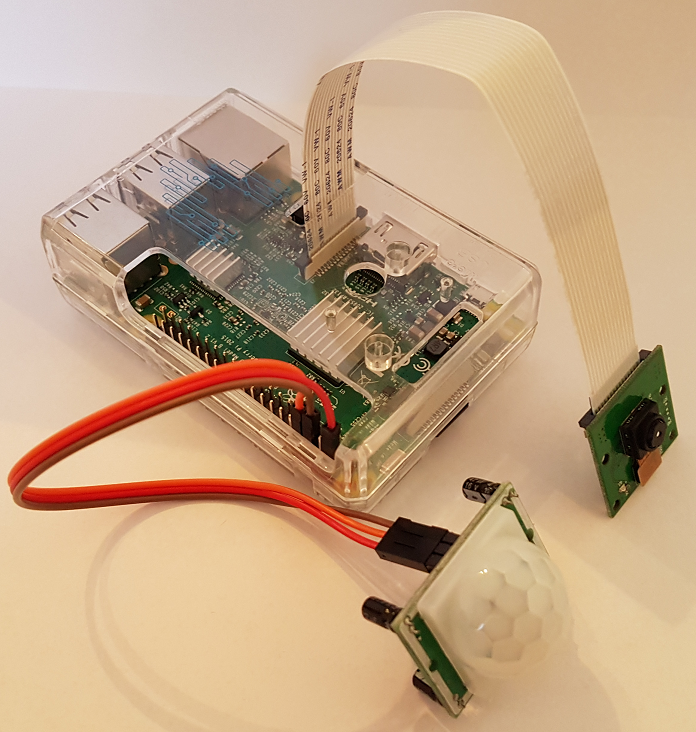
\includegraphics[scale=0.45]{\imageDir/rpisec-hardware-setup.png}
	\caption{Testaufbau der Applikation}
	\label{fig:image-hardware-setup}
\end{figure}
\ \newline
Wie in Abbildung \ref{fig:image-hardware-setup} zu ersichtlich ist, wurde die Kamera über CSI \emph{(Camera-Serial-Interface)}) und der Bewegungssensor über GPIO \emph{(General Purpose Input/Output)} an den \emph{Raspberry PI} angeschlossen.

\subsection{Betriebssysteme}
Dieser Abschnitt behandelt die verwendete Betriebssysteme für den \emph{Raspberry PI}. Die Applikation \emph{RPISec} wurde einerseits mit dem Betriebssystem \emph{hypriotos-rpi} und andererseits mit \emph{Raspian} realisiert. Das Betriebssystem \emph{hypriots} basiert auf \emph{Debian Jessie} und wird von dem \emph{OpenSource} Projekt \emph{hypriot}\footnote{\url{https://blog.hypriot.com/}} zur Verfügung gestellt wird. Das Ziel von \emph{hypriots} ist es ein Betriebssystem für \emph{Raspberry PI} zur Verfügung stellen, das bereits Docker vorinstalliert und betriebsbereit hat. Mit dem Betriebssystem \emph{Raspian} muss Docker selbst installiert, wobei Docker als Paket im \emph{Repository} zur Verfügung steht und daher sich die Installation als unkompliziert gestaltet.
\newline
\newline
Wenn Docker installiert und betriebsbereit ist, dann spielt es keine Rolle auf welchem Betriebssystem die Applikation \emph{RPISec} betrieben wird.
\newline
\newline
Da die Applikation \emph{RPISec} auf eine aktive Internetverbindung angewiesen ist, muss das Betriebssystem so konfiguriert werden, dass der \emph{Raspberry PI} entweder über \emph{Ethernet} oder \emph{Wlan} an ein Netzwerk angebunden ist, das Zugriff auf das Internet erlaubt. In einem produktiven Betrieb muss der \emph{Raspberry PI} über das Internet erreichbar sein, damit die mobilen \emph{Clients} Anfragen an die gehosteten \emph{Microservice} absetzen können.

\section{Software}
Dieser Abschnitt behandelt die verwendete bzw. implementierte Software für \emph{RPISec}.
\subsection{\emph{Microservices} und \emph{Cloud}}
Dieser Abschnitt behandelt die auf dem \emph{Raspberry PI} gehosteten Services. Die Services wurden mit \emph{Spring Boot} als \emph{Microservices} implementiert, was möglich war, da Oracle eine ARM Implementierung der Java-JDK bereitstellt und die \emph{Microservices} schlank implementiert wurden, sodass die zur Verfügung stehenden Ressourcen ausreichen, um diese Services auf einen \emph{Raspberry PI} zu betreiben.
\newline
\newline
Es wurden die beiden \emph{Microservices} \emph{rpisec-auth-service} für die Benutzerverwaltung und OAuth2 Authentifizierung und \emph{rpisec-app-service} für die Interaktion mit der Sensorik und der Interaktion mit dem \emph{Cloud}-Diensten implementiert, wobei der \emph{Microservice} \emph{rpisec-auth-service} im Zuge des Projekts für die Lehrveranstaltung \emph{Service Engineering} implementiert wurde. Es hätte auch ausgereicht die Benutzerverwaltung in den \emph{Microservice rpisec-app-service} zu verpacken, obwohl dann der \emph{Microservice} für zwei Aspekte verantwortlich gewesen wäre was im Widerspruch zu einem \emph{Microservice} steht, der nur für einen Aspekt verantwortlich sein soll. 
\newline
\newline
Der Microservice \emph{rpisec-app-service} interagiert nicht direkt mit der Sensorik, sondern bindet die Sensorapplikation beschrieben in Abschnitt \ref{sec:sensor-application} ein und ist für dessen Lebenszyklus verantwortlich. Nachdem Start der Sensorapplikation wird ein \emph{Listener} registriert, der auf Statusänderungen des Bewegungssensor reagiert und diesen Sicherheitsvorfall wie in Abbildung \ref{fig:image-sequence-incident} behandelt.
\newline
\newline
Die beiden \emph{Microservices} müssen Daten persistent halten und sind daher auf eine Datenbank angewiesen, wobei im Entwicklungsbetrieb auf einen Entwicklerrechner H2 und im produktiven Betrieb auf einen \emph{Raspberry PI} PostgreSQL verwendet wird. Die Datenbank PostgreSQL konnte verwendet werden, da PostgreSQL die ARM Architektur unterstützt.
\newline
\newline
Als \emph{Cloud} Anbieter wurde \emph{Google} gewählt, welcher die Plattform \emph{Firebase} anbietet, die eine JSON-Datenbank und einen \emph{Cloud Messaging} Dienst anbietet. Für diesen Dienst gibt es eine Java Implementierung das sogenannte \emph{firebase-admin-sdk}, das eine API zum Interagieren mit der JSON-Datenbank und eine API zum Erstellen von Authentifizierungstoken für die \emph{Client}-Authentifizierung bei Firebase zur Verfügung stellt. In der Java Implementierung wird zurzeit keine API für die Interaktion mit dem \emph{Messaging} Dienst zur Verfügung gestellt, was aber kein Problem darstellt, da es sich hierbei um eine einfache Anfrage an eine \emph{REST-API} handelt, die mit Spring \emph{RestTemplate} durchgeführt wird.
\subsection{Sensor Applikation}

Bei den Komponenten der Sensor-Anwendung handelt es sich, wie in \autoref{sec:raspberrypi} erwähnt, um die beiden Bauteile:

\begin{itemize}
	\item \emph{AZDeliveryCamRasp Kamera}
	\item \emph{HC-SR501 Bewegungssensor}
\end{itemize}

\subsection{Kamera}

Bei der Kamera handelt es sich um ein eigens für den Raspberry Pi entwickeltes Modell und wird direkt an den vorhanden Kamera-Port des Raspberry Pi 3\footnote{\url{https://en.wikipedia.org/wiki/Raspberry_Pi\#/media/File:Raspberry-Pi-3-Flat-Top.jpg}} angeschlossen.

\begin{figure}[h]
	\centering
	\includegraphics[scale=0.20]{\imageDir/rpi-border-cam.jpg}
	\caption{Raspberry-Pi 3}
	\label{fig:rpi-border-cam}
\end{figure}

Anschließend muss die Kamera aktiviert werden. Dies geschieht über das, mit den meisten Linux-Distributionen mitgelieferte, Programm \emph{raspi-config\footnote{\url{https://upload.wikimedia.org/wikipedia/commons/e/ed/Raspi-config.png}}}. Dieses Programm wird auch benutzt um andere Komponenten des Raspberry Pi zu konfigurieren.

\begin{figure}[h]
	\centering
	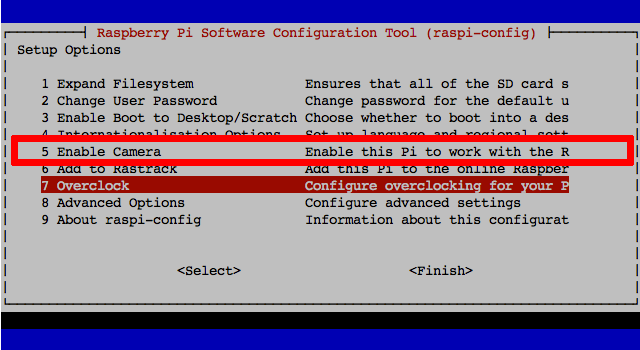
\includegraphics[scale=0.40]{\imageDir/raspi-config-cam.png}
	%By Onepiece84 (Own work) [CC BY-SA 4.0 (http://creativecommons.org/licenses/by-sa/4.0)], via Wikimedia Commons
	\caption{Raspi-config}
	\label{fig:raspi-config-cam}
\end{figure}

Zur Ansteuerung der Kamera wird das Konsolenprogramm \emph{raspistill} verwendet. Diese kann mit verschiedensten Parametern konfiguriert werden. Als Beispiel:\\
\newline
\begin{code}
	raspistill --width 1920 --height 1080 -o test.jpg\\
\end{code}
\newline
Dies erzeugt ein Bild in der Auflösung 1920 x 1080 Pixel und speichert es unter dem Dateinamen \emph{test.jpg}.

\subsection{HC-SR501 Bewegungssensor}

Der HC-SR501 Sensor wird über die GPIO-Pins des Raspberry Pi angesteuert. Hierbei werden Masse, Stromversorgung und Daten-Pin des HC-SR501 Sensors mit den GPIO-Pins verbunden. 

\begin{figure}[h]
	\centering
	\includegraphics[scale=0.20]{\imageDir/rpi-border-gpio.jpg}
	\caption{Raspberry-Pi 3}
	\label{fig:rpi-border-gpio}
\end{figure}

Die Pin-Belegung\footnote{\url{http://www.netzmafia.de/skripten/hardware/RasPi/Projekt-PIR/}} des HC-SR501

\begin{figure}[h]
	\centering
	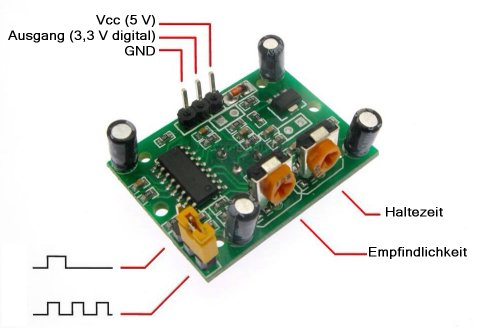
\includegraphics[scale=0.50]{\imageDir/PIR4.jpg}
	\caption{Pin-Schema HC-SR501}
	\label{fig:PIR4}
\end{figure}

ist wie folgt definiert:

\begin{itemize}
	\item Pin 1: VCC (5 Volt)
	\item Pin 2: Out, Data
	\item Pin 3: GND, Masse
\end{itemize}

zusätzlich kann die Empfindlichkeit und Haltezeit an den beiden Drehreglern eingestellt werden. Zusätzlich kann noch das Daten-Pin Verhalten über den Jumper konfiguriert werden.

\pagebreak

\subsection{GPIO}

GPIO ist die Abkürzung für General Purpose Input Output. Man bezeichnet damit programmierbare Ein- und Ausgänge für allgemeine Zwecke. Die GPIOs werden als Lötpunkt oder Pin in Form einer Stiftleiste herausgeführt und dienen als Schnittstelle zu anderen Systemen oder Schaltungen, um diese über den Raspberry Pi zu steuern. Dabei kann der Raspberry Pi bei entsprechender Programmierung digitale Signale von außen annehmen (Input) oder Signale nach außen abgeben (Output).\\

Viele der GPIOs erfüllen je nach Einstellung und Programmierung verschiedene Funktionen. Neben den typischen GPIO-Ein- und Ausgängen finden sich aber auch Pins mit der Doppelfunktion für I2C, SPI und eine serielle Schnittstelle.\\

\subsubsection{HC-SR501 GPIO Verbindung}

Für den HC-SR501 wird die Pin-Belegung wie folgt gewählt:

\begin{itemize}
	\item Pin 1: VCC (5 Volt) an Pin 2
	\item Pin 2: Out, Data an Pin 8
	\item Pin 3: GND an Pin 6
\end{itemize}

Diese Pin-Belegung erfolgt aufgrund der folgenden schematischen Darstelleung\footnote{\url{http://pi4j.com/pins/model-3b-rev1.html}}:

\begin{figure}[h]
	\centering
	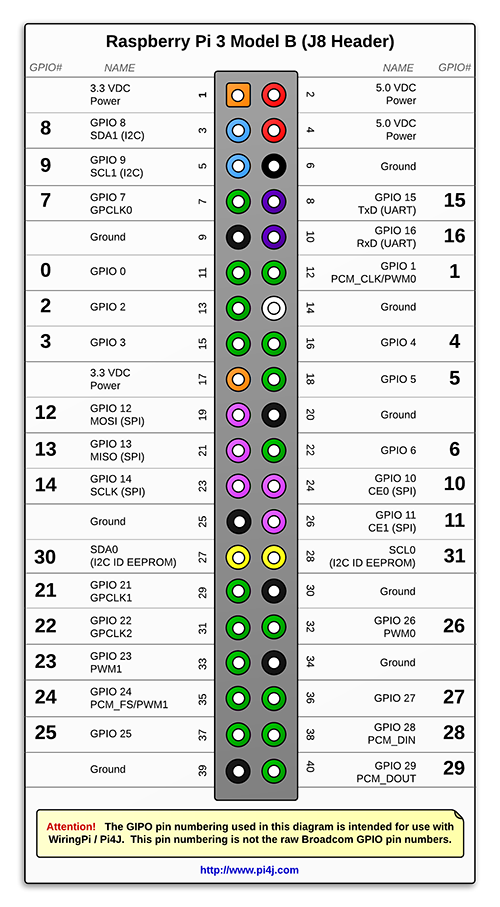
\includegraphics[scale=1.00]{\imageDir/j8header-3b.png}
	\caption{Pin-Schema}
	\label{fig:j8header-3b}
\end{figure}

\pagebreak

\subsection{Pin-Ansteuerung mit Java}

Die Ansteuerung der Pins erfolgt über die \emph{Pi4J\footnote{\url{http://pi4j.com/}}}-Bibliotheken die wiederum die \emph{WiringPi\footnote{\url{http://wiringpi.com/}}}-Bibliothek nutzt, welche die eigentliche Ansteuerung der Pins erledigt.

\subsubsection{Pi4J}
Pi4J ist eine Bibliothek  für Java, die den vollen Zugriff auf die Ressourcen des Raspberry PI ermöglicht. Mit Pi4J ist es möglich Anwendungen für Raspberry PI zu schreiben, die nur Java benötigen. Damit können praktisch alle Bibliotheken eingesetzt werden, die für Java verfügbar sind. Einschränkungen gibt es nur bei den Ressourcen des Raspberry.

\subsubsection{WiringPi}
WiringPi ist ein nützliches Framework um die GPIO Ein-und Ausgänge am Raspberry Pi zu schalten. Das Ziel dieser Bibliothek ist es, eine einzige gemeinsame Plattform und Programmierschnistelle für den Zugriff auf die GPIOs des Rapsberry Pi für verschiedene Programmiersprachen zur Verfügung zu stellen. Im Kern ist WiringPi eine C-Bibliothek, aber sie steht auch in Ruby und Python zur Verfügung.

\begin{code}
	\caption{gpio-controller.java}
	\yamlFile{\srcDir/gpio-controller.java}
	\label{src:gpio-controller}
\end{code}
\subsection{Mobiler \emph{Client}}


% Quellen
% AZDeliveryPICam:
% https://www.amazon.de/dp/B01M6UCEM5/ref=pe_386171_51767411_TE_dp_3
% -------------------------------------------------------------------
% HC-SR501
% https://www.amazon.de/dp/B00TI2ZC72/ref=pe_386171_38075861_TE_item
% -------------------------------------------------------------------
% HC-SR501 Schema
% ttp://www.netzmafia.de/skripten/hardware/RasPi/Projekt-PIR/
% -------------------------------------------------------------------

\end{document}          
